\subsection{Administrationssystem}
Dette delsystem indeholder al funktionalitet til at manipulere produkter og produktkategorier. Dette indebærer oprettelse, sletning og redigering af produkterne og produktkategorierne. Administrationsystem er koblet op til CentralServer, og kommunikerer med denne via en Socket forbindelse (TCP/IP).

\subsubsection{Designovervejelser}
Designet af Administrationssystem startede ud med at lave en skitsering af, hvordan det grafiske skulle se ud. Dette betød at der skulle udvikles en grov skitse af designet\footnote{Skitse af designet kan ses i dokumentationen, side XYZ}.\\
Selve softwaren til Administrationssystem skulle sættes op på en måde, så det var overskueligt og modulært. I software design kurset blev der givet undervisning i designprincippet MVVM~\cite{MVVM}, som forklarer, hvordan man kan dele sin GUI-applikation op og adskille funktionalitet fra præsentation. Præsentation er det rent visuelle, altså opsætning af knapper, tekstbokse og så fremdeles. Funktionaliteten er den bagvedliggende hjerne i applikationen.\\
Administrationssystem softwaren var først lavet med funktionaliteten i codebehind\footnote{C\#-filen til XAML viewet (WPF)}, hvilket hurtigt blev både komplekst, rodet og ikke mindst skabte en høj kobling. Der blev da senere undervist i MVVM-designmønstret, hvorefter det blev besluttet at refaktorere til brug af MVVM designmønstret.\\
Det visuelle design og funktionaliteten til at vise produkter og kategorier blev lavet i starten af udviklingen. Efter dette skulle kommunikationen mellem Administrationssystem og CentralServer på plads. Implementeringen af CentralServer satte en standard for, hvordan og hvornår data blev sendt frem og tilbage mellem CentralServer og de andre delsystemer, og derfor skulle der blot laves kommunikation for Administrationssystem der opfyldte disse krav. Det primære krav var, at Administrationssystem kontinuert skulle lytte på indkommende data, da der kunne blive sendt vigtig data på alle tidspunkter, også selvom den pågældende instans af Administrationssystem ikke havde anmodet CentralServer om noget.

\subsubsection{Implementering}
Det endelige design af Administrationssystemet er implementeret med MVVM som det primære design. Designet af den grafiske brugerflade holder sig op af det skitserede design.\\
Administrationssystem fungerer sådan, at ved start af programmet åbnes et hovedvindue, der viser systemets nuværende produkter samt produktaktegorier. Herfra er der knapper til resten af programmets funktionalitet, som indebærer opret, rediger og slet af produkter og kategorier. Produkter og kategorier kan markeres på den pågældende liste og ved sletning eller redigering slettes/ændres der på det markerede element.\\

\begin{figure}[H]
	\centering
	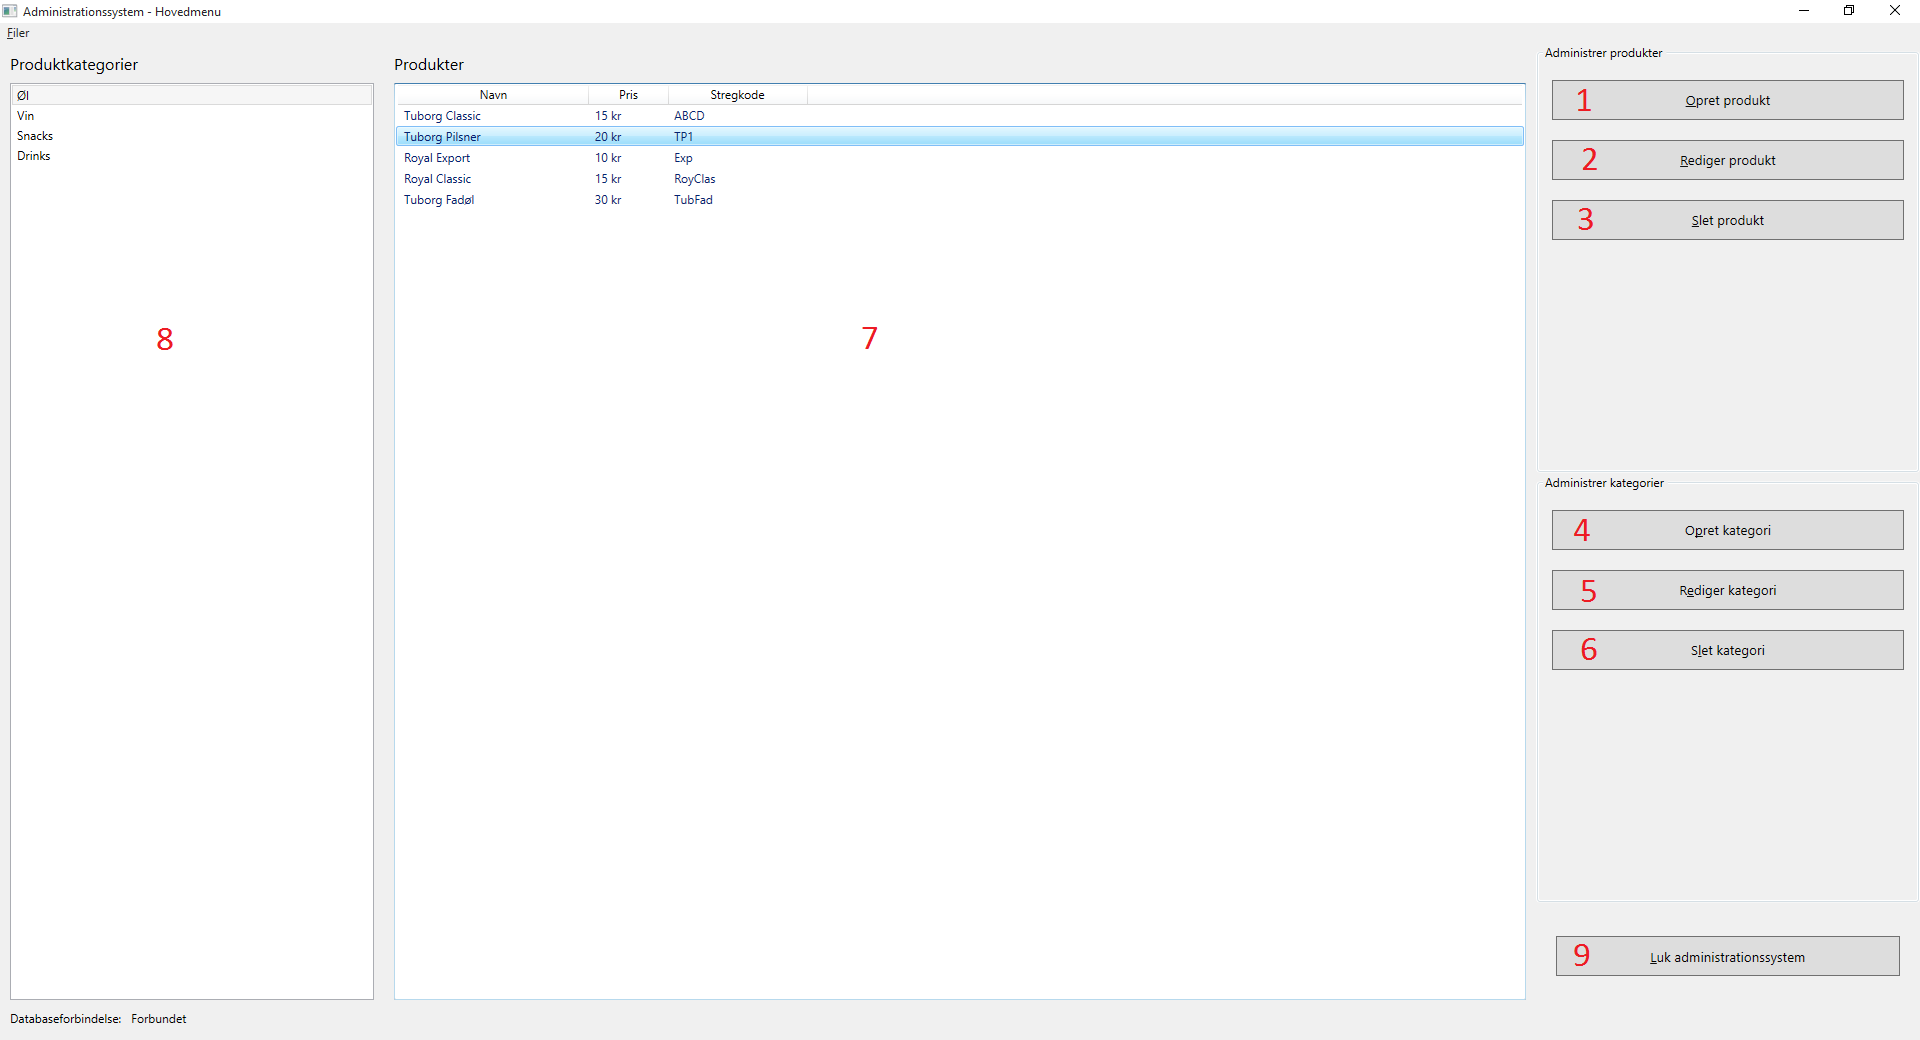
\includegraphics[width=\textwidth]{Projektbeskrivelse/DesignOgImplementering/Images/BackendDemo}
	\caption{Hovedvinduet i Administrationssystem}
	\label{fig:admindemo}
\end{figure}

Figur \ref{fig:admindemo} viser det endelige design af Administrationssystemets hovedvindue. Vinduets elementer er markeret med tal. Forklaring følger:
\begin{enumerate}
	\item Knap til at oprette et nyt produkt. Åbner et nyt vindue.
	\item Knap til at redigere et eksisterende produkt. Der skal være markeret et produkt på produktlisten (se punkt 7) for at knappen kan anvendes. Åbner et nyt vindue.
	\item Knappen til at slette et produkt. Der skal ligeledes være et produkt markeret for at anvende knappen. Åbner blot en popup-meddelelse, hvor der skal vælges ja eller nej.
	\item Knap til at oprette en produktkategori. Åbner et nyt vindue.
	\item Knap til at redigere en produktkategori. Der skal være en produktkategori markeret før knappen er anvendelig. Åbner et nyt vindue.
	\item Knap til at slette en produktkategori. Der skal være markeret en produktkategori for at knappen kan anvendes. Åbner et nyt vindue.
	\item Dette er produktlisten for den valgte kategori (se punkt 8).
	\item Dette er kategorilisten. Når der vælges en kategori på denne liste, så vil kategoriens produkter blive vist på produktlisten (punkt 7).
\end{enumerate}

\textbf{Kommunikation}\\
Kommunikationen mellem Administrationssystem og CentralServer har to dele. Den første er at sende data til CentralServer, den anden er at modtage data. Den data der sendes og modtages er i XML-format. Et eksempel på data der bliver sendt og modtaget mellem Administrationssystem og CentralServer kan ses på nedenstående sekvensdiagram, figur \ref{fig:adminsekvens}.

\begin{figure}[H]
	\centering
	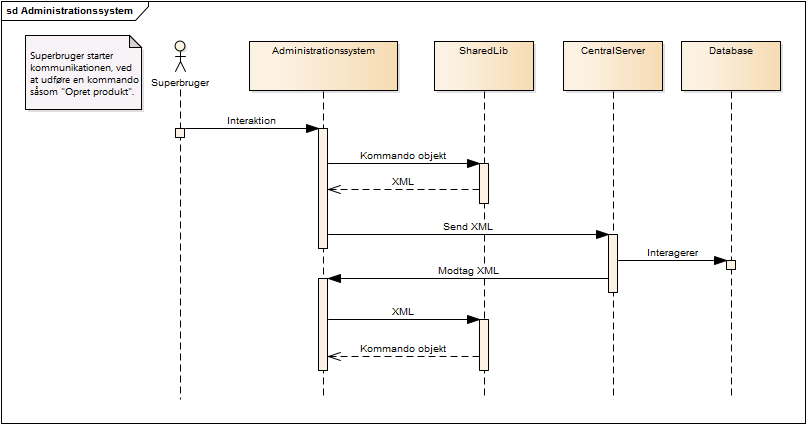
\includegraphics[width=0.8\textwidth]{Projektbeskrivelse/DesignOgImplementering/Images/Administrationssystem-sekvensdiagram}
	\caption{Kommunikation mellem Administrationssystem og CentralServer}
	\label{fig:adminsekvens}
\end{figure}

Figur \ref{fig:adminsekvens} viser et eksempel på, hvad der foregår, når brugeren eksempelvis opretter et nyt produkt. Brugeren foretager en handling i brugergrænsefladen og trykker gem, herefter laves en kommando, som laves til en XML-streng ved hjælp af SharedLib. Denne streng sendes til serveren. Serveren modtager og dekoder XML strengen, foretager handlinger på databasen og sender et svar tilbage i XML format.\\
Når Administrationssystem modtager data vil XML-strengen prøvet at blive dekodet. Hvis strengen indeholder en hel kommando vil der blive foretaget en handling ud fra denne kommando. Kommandoerne der modtages indeholder funktioner der fortæller om et produkt er oprettet, redigeret eller slettet og det samme for kategorier. Dette betyder, at uanset hvornår Administrationssystem modtager en kommando, så vil produkt- og kategorilister blive opdateret.\\
Ved at bruge benytte denne måde at modtage data på, garanteres det, såfremt der er forbindelse fra Administrationssystem til CentralServer, at Administrationssystem altid vil være synkront med databasen - også selvom et andet Administrationssystem har oprettet et nyt produkt eller produktkategori.
